\chapter[Estudo Exploratório]{Estudo Exploratório}

Para a realização da proposta foi adotada a atividade de exploração, devido ao grau de intervenção foi baixo. O paradigma empregado foi experimental e a análise realizada foi semi-quantitativa, pois associou-se observação a medição de alguma tendência. Os passos adotados foram, em sua maioria, os sugeridos por \citeonline{travassos2011experimentaccao}. O estudo exploratório foi concebido com base nos objetivos levantados na proposta de estudo \ref{propostaestudo}, e em cada foi conduzido. Na Seção \ref{sec:planejamento} consta a descrição de como o estudo foi preparado. As etapas de execução estão na Seção \ref{sec:execucao}, seguido pelos resultados presentes na Seção \ref{sec:resultados} e por fim, a análise e discussão está na Seção \ref{sec:discussao}.

\section{Planejamento \label{sec:planejamento}}

Para conseguir a realização do estudo exploratório foi necessário planejar três principais aspectos: a geração de dados de teste, a execução da cobertura de código e o parâmetro de estudo, ou seja, o código no qual as etapas anteriores utilizaria.

A princípio, buscou-se trabalhar com o menor escopo possível, escolhendo um algoritmo genético simples que se assemelha a definição formal. E a partir disso definir uma função objetivo para a geração de dados de teste. O algoritmo adotado foi o presente no livro de \cite{russell2016artificial}, e o parâmetro de estudo escolhido foi o \textit{Scikit-learn} \cite{pedregosa2011scikit}. Nas primeiras manipulações, foi constatado que seria um trabalho fastidioso e que não estaria de acordo com a proposta de estudo. Por isso, contornou-se o planejamento para a escolha de uma ferramenta de geração de dados de teste que está em um estado mais avançado. 

A seleção aconteceu ao se consultar a competição de ferramentas para testes unitários em Java, que teve sua quinta edição em 2017 e faz parte do congresso de SBST \cite{panichella2017java}. Foi escolhido então, a ferramenta EVOSUITE\footnotemark \footnotetext{\url{http://www.evosuite.org/}}, ganhadora da última edição, que gera automaticamente casos de teste com asserções para classes escritas em código Java \cite{fraser2011evosuite}. 

A EVOSUITE aplica uma abordagem multiobjetivo para os critérios de busca, ou seja, constrói a função objetivo da otimização baseando em mais do que no critério de cobertura de código. Adicionalmente, ela possui uma série de parâmetros para a execução, como a seleção de qual algoritmo utilizar, visto que tem suporte mais de um, o tempo de busca para otimização, a quantidade máxima de iterações, o tamanho da população, no caso dos algoritmos genéticos, entre outros. 

Como parâmetro de estudo foi escolhido o projeto Jsoup\footnotemark \footnotetext{\url{https://jsoup.org/}}, que é uma biblioteca Java para trabalhar com HTML, que fornece uma API para extrair e manipular dados de páginas web. É um projeto de código livre fácil de manipular e compreender \cite{hedley2009jsoup}. Além disso, ela maior se adequa a EVOSUITE por ser orientada a objeto e por estar em Java. Uma opção melhor, mas que prejudicaria bastante os testes por causa do tempo de teste é o conjunto de projetos denominado de SF100 \cite{TOSEM_evaluation}, criado especialmente para teste de integração das novas versões do EVOSUITE.

Com a definição da ferramenta e do projeto, partiu-se então para o planejamento da execução dos experimentos de exploração. De acordo com o propósito, viu-se a necessidade de ter várias massas de dados que se distinguem no tempo. Assim, sendo a geração de dados de teste e a execução dos mesmos serão realizados a cada período de tempo acrescido. A estratégia será adotada justamente para se conseguir observar o comportamento de tais atividades.

\section{Execução \label{sec:execucao}}

A execução do estudo exploratório fez uso adicional das seguintes ferramentas:

\begin{enumerate}
    \item OpenClover\footnotemark \footnotetext{\url{http://openclover.org/}}: ferramenta de cobertura de código para Java, Groovy e AspectJ.
    \item Matplotlib\footnotemark \footnotetext{\url{https://matplotlib.org/}}: biblioteca de plotagem de gráficos 2D em Python.
    \item Pandas\footnotemark \footnotetext{\url{https://pandas.pydata.org/}}: biblioteca que fornece estruturas de dados de alto desempenho e ferramentas de análise de dados para a linguagem de programação Python.
\end{enumerate}

O OpenClover foi selecionado devido a sua facilidade de customização da execução e de extração dos dados de cobertura de código. A adoção do Matplotlib junto com o Pandas se deve a simplicidade de construção do tipo de gráfico escolhido. Todas as ferramentas utilizadas são gratuitas e de código aberto.

O passo a passo da execução dos experimentos podem ser vistos abaixo. Foram criados scripts (\ref{scripts}) que sistematizaram e garantiram a replicabilidade dos procedimentos. Eles foram executados em um ambiente computacional com o processador Intel Core i7-7700 CPU @3.60GHz e com 16GB de memória RAM.

\subsection{Execução dos ensaios de teste}

Etapa em que o script run.sh (\ref{run.sh}) é executado. A sua aplicação é realizada na pasta anterior ao do projeto em que vai se executar a ferramenta EVOSUITE, da seguinte maneira: \mintinline{shell}{./run.sh TARGET_CLASS PATH_PROJECT SUBPATH_PROJECT}. É necessário a passagem de três parâmetros, o \mintinline{shell}{TARGET_CLASS} que é o nome da classe incluindo o pacote que vai ser executado, o \mintinline{shell}{PATH_PROJECT} que se refere a pasta do projeto que vai ser testado e o \mintinline{shell}{SUBPATH_PROJECT} que é a estrutura de diretório que o projeto se encontra. 

Um exemplo do script para a classe \textit{Parser} do pacote \textit{parser} que é testada e a cobertura de código verificada executado é o seguinte: 

\mintinline{shell}{./run.sh org.jsoup.parser.Parser jsoup org/jsoup/parser}

Em cada ensaio, são executadas 10 massas de dado que variam de 2 em 2 segundos até o limite de 20 segundos. Tal parâmetro é \mintinline{shell}{-Dsearch_budget}, que e a propriedade de execução do EVOSUITE que delimita o tempo de busca do algoritmo. Com a geração dos testes pela ferramenta, é executada a cobertura com o OpenClover que vai guardando o histórico em um diretório diferente do projeto. O EVOSUITE, por sua vez, cria o diretório \textit{evosuite-report} e armazena as estatísticas no arquivo \textit{statistics.csv}.

\subsection{Extração das métricas da execução da cobertura de código}

Essa etapa é responsável for extrair as métricas de tempo e cobertura de código a partir dos relatórios salvos pelo OpenClover durante a etapa anterior. Para isso, foi criado o script \mintinline{shell}{./extract.sh} (\ref{extract.sh}), que é executado no diretório \textit{clover-history} e produz o arquivo \textit{statistics-execution.csv}. 

Um detalhe dessa etapa é que a cobertura pela ferramenta se dá pela divisão dos elementos cobertos pelo total de elementos. O elemento no caso são os critérios de cobertura da OpenClover, que vão além de a quantidade de linhas do programa.

\subsection{Manipulação dos dados}

Essa etapa é bem simples, consiste apenas na extração manual do dados específicos da classe que se deseja do arquivo \textit{statistics.csv} produzido pelo EVOSUITE. Isso porque, ele guarda o histórico de todas as execuções. Um passo importante também e retirar o aquivo anteriormente produzido (\textit{statistics-execution.csv}) para o diretório aonde os gráficos serão gerados.

\subsection{Geração dos gráficos} 

Para a geração dos gráficos foi produzido o script em Python \textit{plot.py} (\ref{plot.py}). Sua execução necessita do nome do arquivo, que por padrão adotou-se o nome da classe e o tipo, sendo geração ou execução (\mintinline{python}{python plot.py FILENAME TYPE}). Abaixo segue o exemplo para a classe \textit{Parser}:

\mintinline{python}{python plot.py jsoup.parser.parser generation} 
 
\mintinline{python}{python plot.py jsoup.parser.parser execution}

\section{Resultados \label{sec:resultados}}

A princípio, não obedecendo os passos anteriormente citados, foi realizado um ensaio com todas as classes do pacote \textit{parser}

\begin{figure}[H]
	\centering
	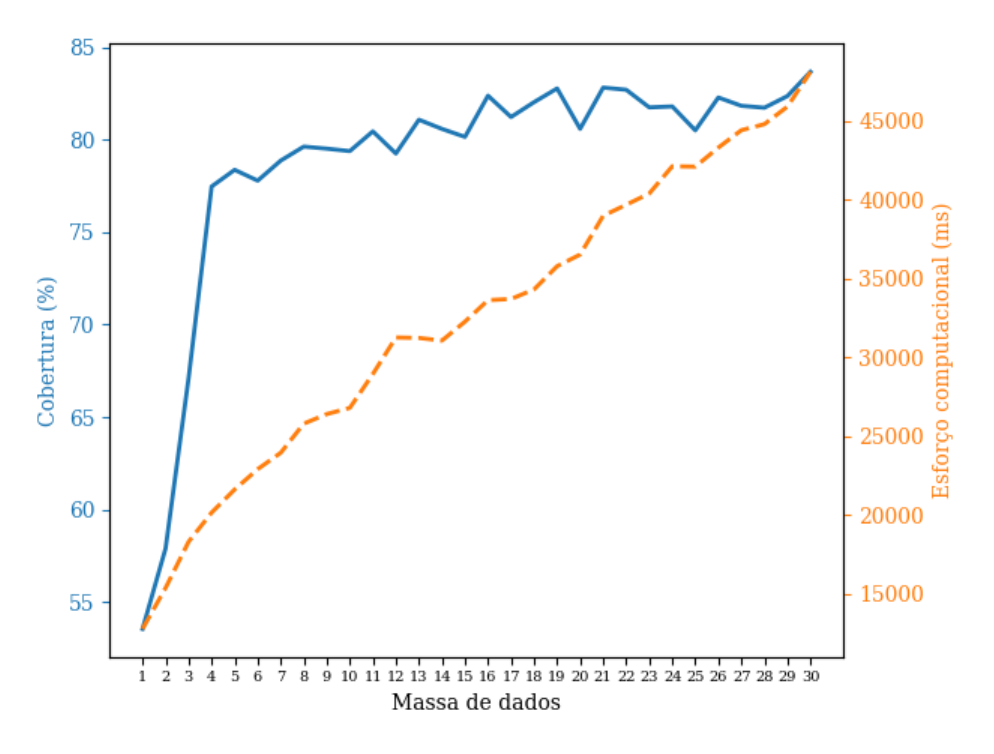
\includegraphics[scale=0.6]{figuras/jsoup.parser_generation.eps}
	\caption{Geração de dados de teste para o pacote \textit{jsoup.parser}}
	\label{fig:genJsoup}
\end{figure}

\begin{figure}[H]
\centering
\begin{subfigure}{.5\textwidth}
    \centering
    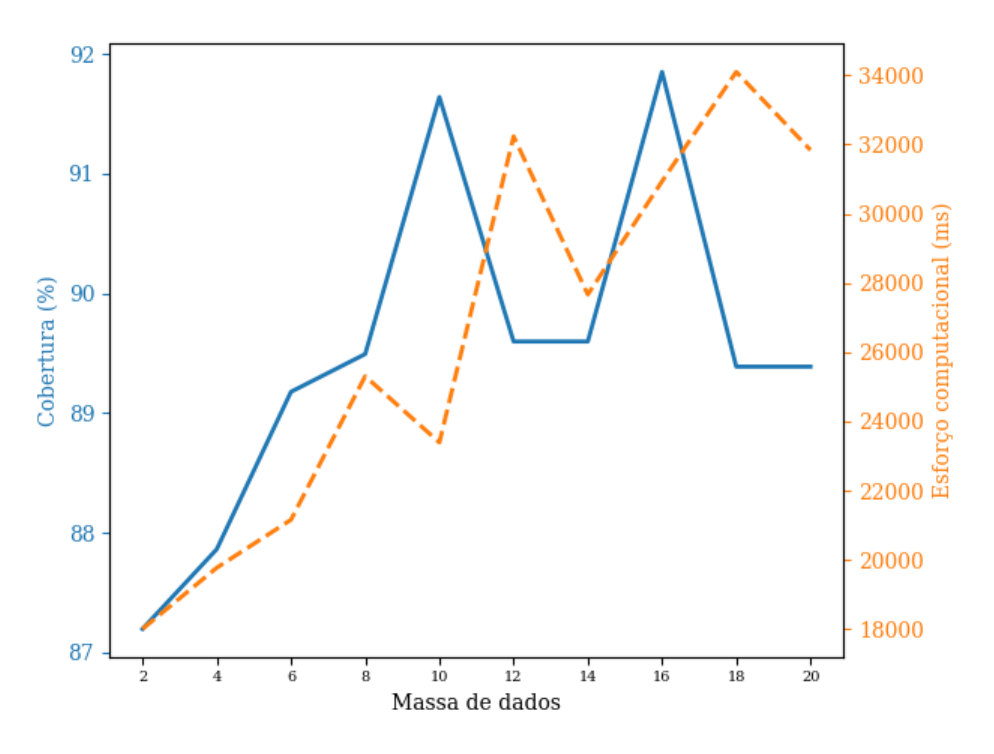
\includegraphics[scale=0.5]{figuras/jsoup.parser.parser_generation.eps}
    \caption{Geração dos testes}
    \label{fig:genJsoupParser}
\end{subfigure}%
\begin{subfigure}{.5\textwidth}
    \centering
    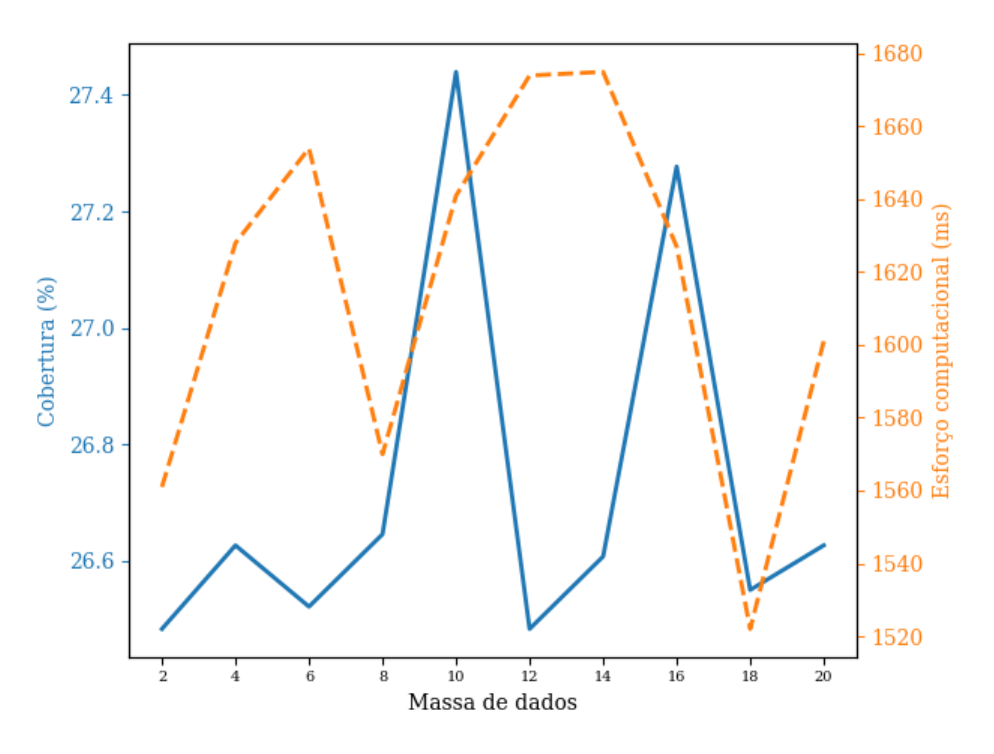
\includegraphics[scale=0.5]{figuras/jsoup.parser.parser_execution.eps}
    \caption{Execução dos testes}
    \label{fig:execJsoupParser}
\end{subfigure}
\caption{Classe \textit{jsoup.parser.Parser}}
\label{fig:JsoupParser}
\end{figure}


% \begin{figure}[H]
% 	\centering
% 	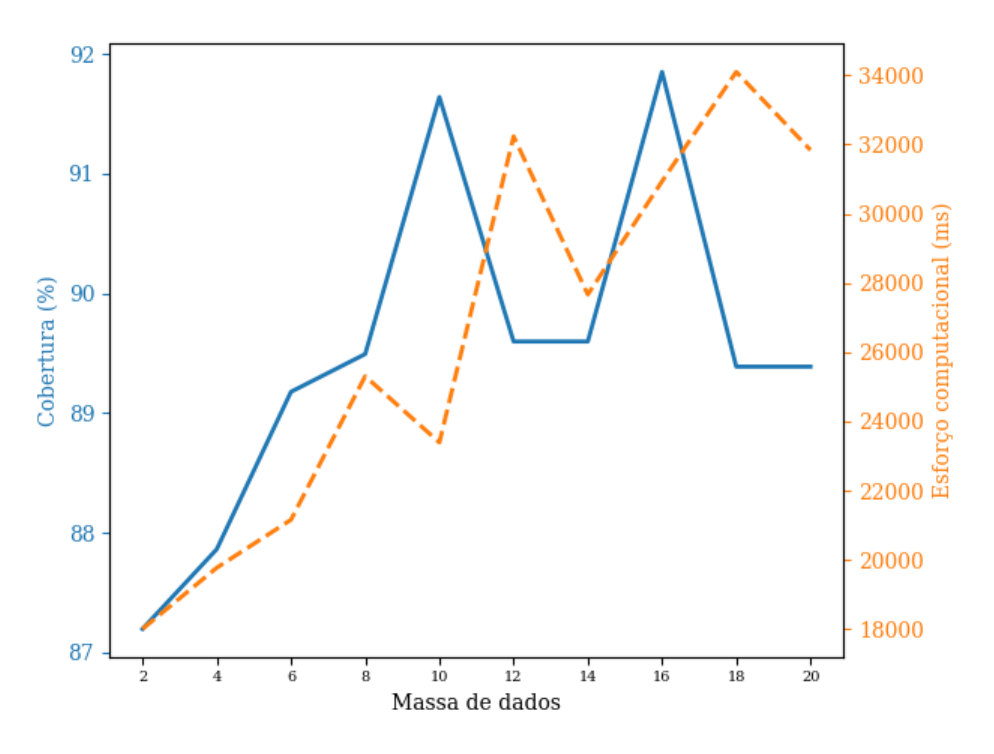
\includegraphics[scale=0.6]{figuras/jsoup.parser.parser_generation.eps}
% 	\caption{Geração de dados de teste para a classe \textit{jsoup.parser.Parser}}
% 	\label{fig:genJsoupParser}
% \end{figure}

% \begin{figure}[H]
% 	\centering
% 	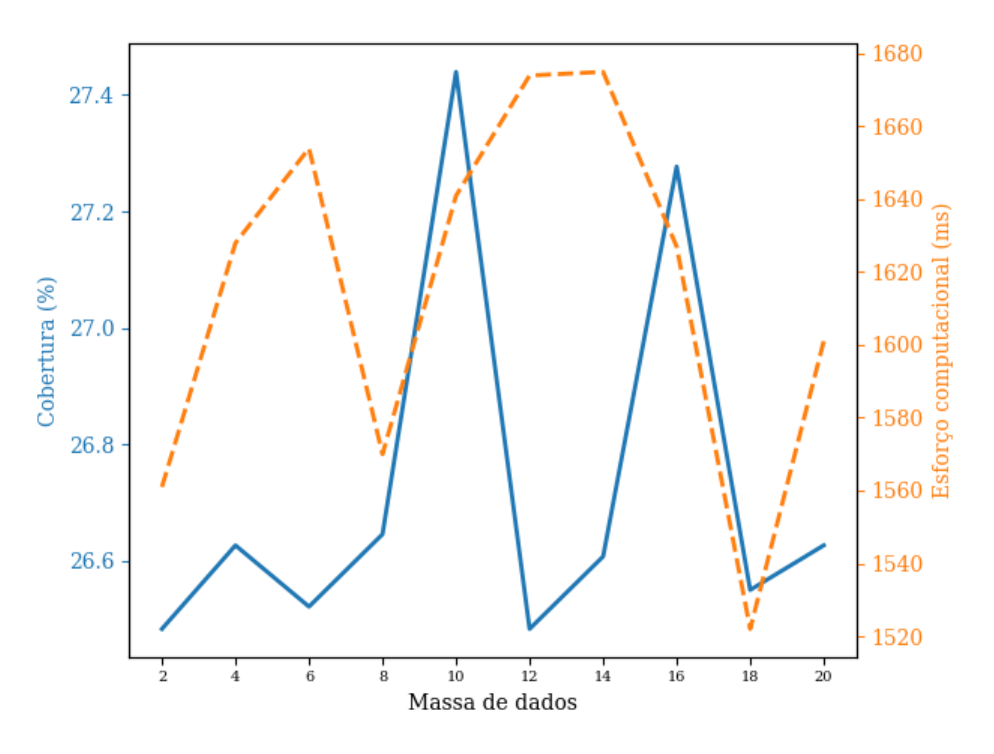
\includegraphics[scale=0.6]{figuras/jsoup.parser.parser_execution.eps}
% 	\caption{Execução dos teste da classe \textit{jsoup.parser.Parser}}
% 	\label{fig:execJsoupParser}
% \end{figure}

\begin{figure}[H]
    \centering
    \begin{subfigure}{.5\textwidth}
        \centering
        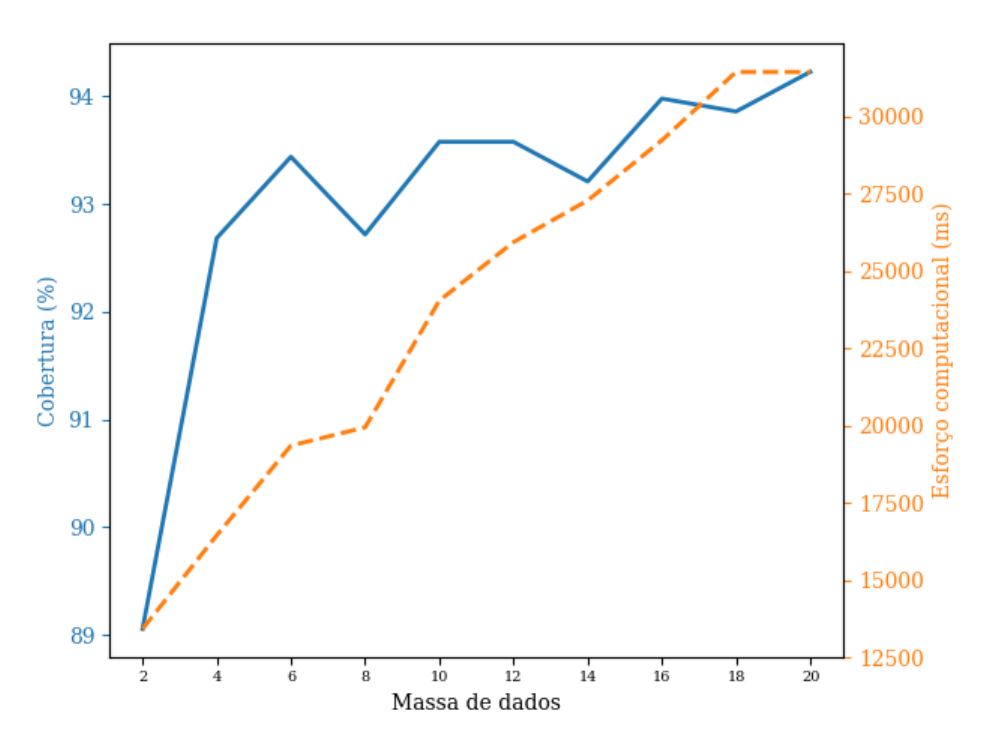
\includegraphics[scale=0.5]{figuras/jsoup.parser.tag_generation.eps}
        \caption{Geração dos testes}
        \label{fig:genJsoupTag}
    \end{subfigure}%
    \begin{subfigure}{.5\textwidth}
        \centering
        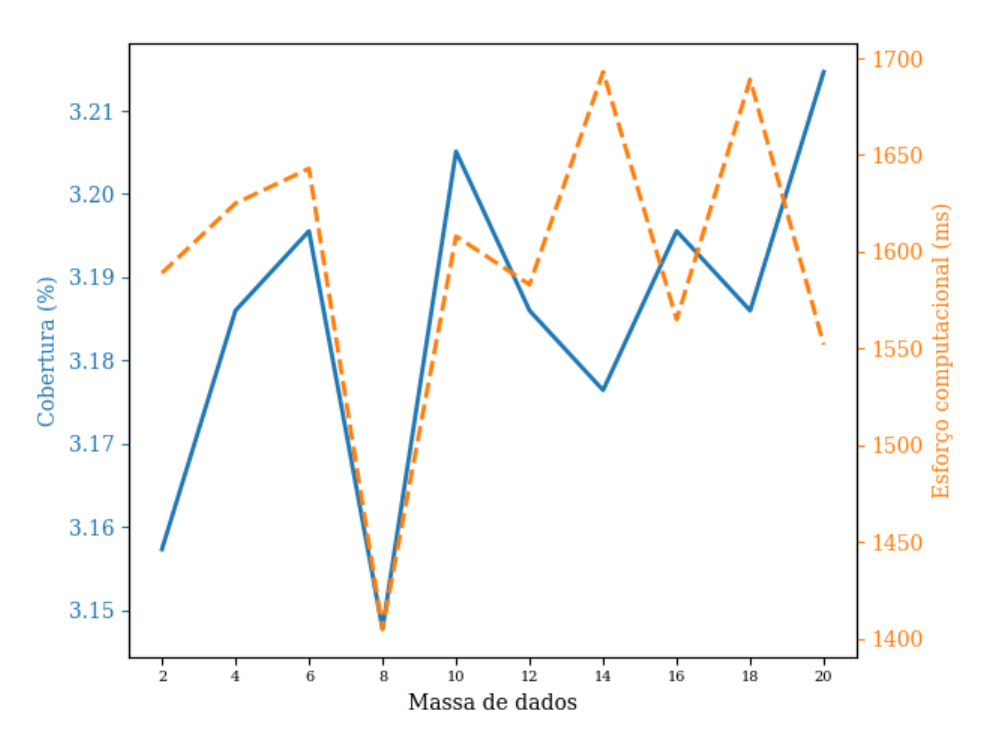
\includegraphics[scale=0.5]{figuras/jsoup.parser.tag_execution.eps}
        \caption{Execução dos testes}
        \label{fig:execJsoupTag}
    \end{subfigure}
    \caption{Classe \textit{jsoup.parser.Tag}}
\label{fig:test}
\end{figure}

% \begin{figure}[H]
% 	\centering
% 	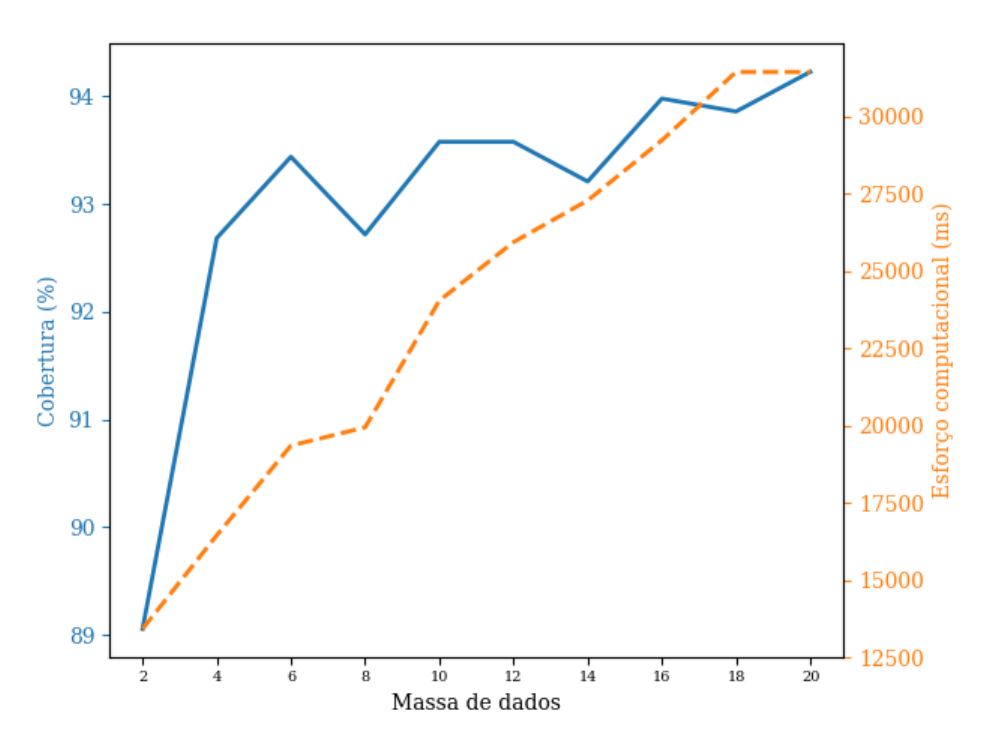
\includegraphics[scale=0.6]{figuras/jsoup.parser.tag_generation.eps}
% 	\caption{Geração de dados de teste para a classe \textit{jsoup.parser.Tag}}
% 	\label{fig:genJsoupTag}
% \end{figure}

% \begin{figure}[H]
% 	\centering
% 	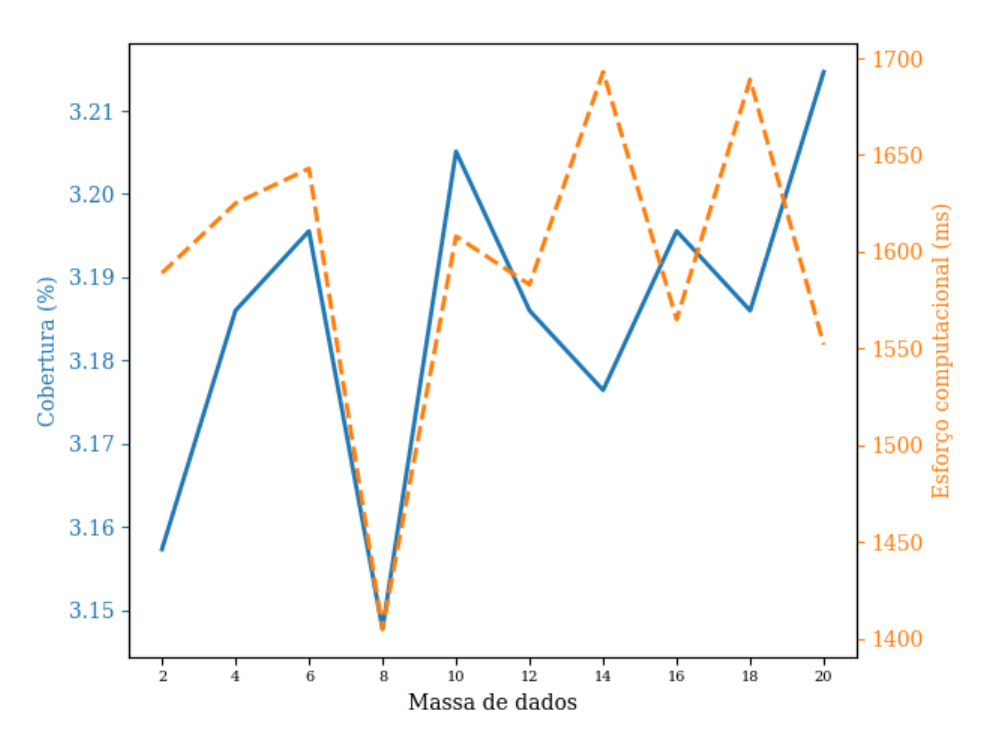
\includegraphics[scale=0.6]{figuras/jsoup.parser.tag_execution.eps}
% 	\caption{Execução dos teste da classe \textit{jsoup.parser.Tag}}
% 	\label{fig:execJsoupTag}
% \end{figure}


\begin{figure}[H]
    \centering
    \begin{subfigure}{.5\textwidth}
        \centering
        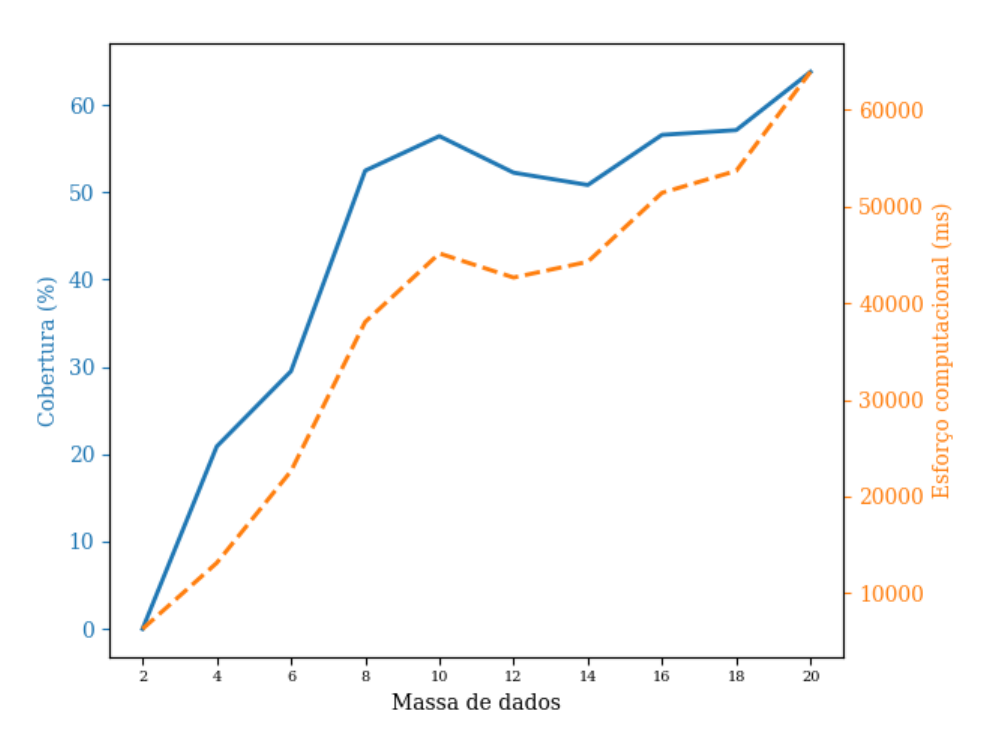
\includegraphics[scale=0.5]{figuras/jsoup.parser.htmltreebuilder_generation.eps}
        \caption{Geração dos testes}
        \label{fig:genJsoupHtmlTreeBuilder}
    \end{subfigure}%
    \begin{subfigure}{.5\textwidth}
        \centering
        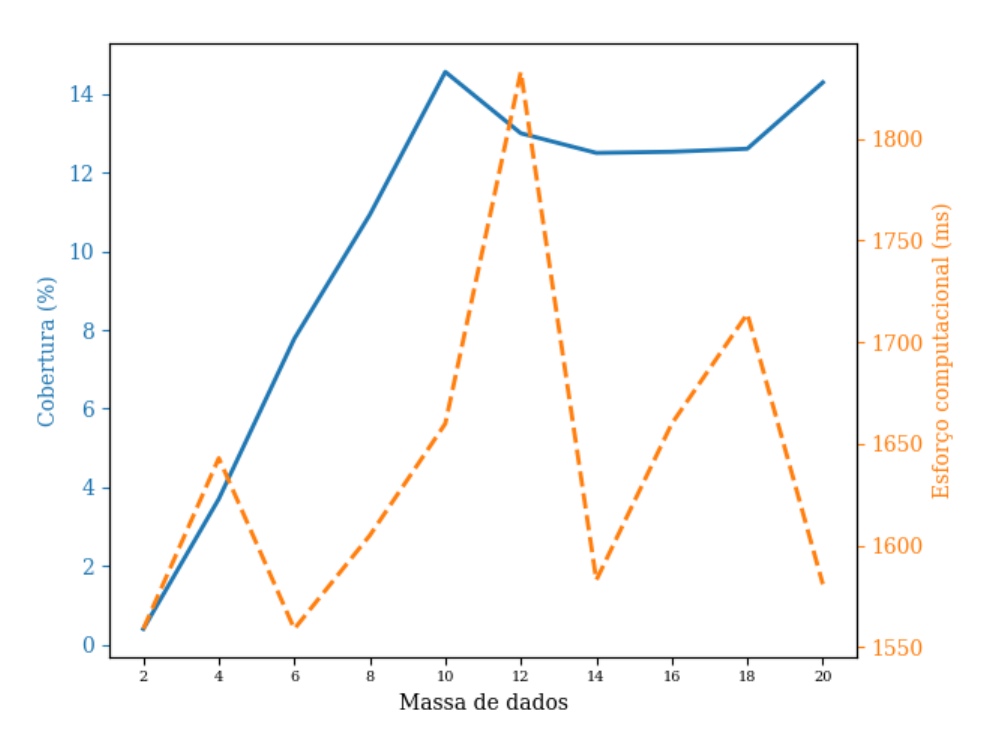
\includegraphics[scale=0.5]{figuras/jsoup.parser.htmltreebuilder_execution.eps}
        \caption{Execução dos testes}
        \label{fig:execJsoupHtmlTreeBuilder}
    \end{subfigure}
    \caption{Classe \textit{jsoup.parser.HtmlTreeBuilder}}
\label{fig:JsoupHtmlTreeBuilder}
\end{figure}

\section{Discussão \label{sec:discussao}}

\subsection{Ameaças a Validade}

